\documentclass[11pt]{article}

\usepackage[margin=1in, headheight=14.5pt]{geometry}
\usepackage{amsfonts, amsmath, amssymb}
\usepackage[none]{hyphenat}
\usepackage{fancyhdr}
\usepackage[spanish]{babel}
\usepackage[spanish, calc]{datetime2}
\usepackage{fmtcount}
\usepackage{graphicx}
\usepackage{float}
\usepackage[nottoc, notlot, notlof]{tocbibind}
\usepackage{tocloft}
\usepackage[utf8]{inputenc}
\usepackage{parskip}
\usepackage{xcolor}
\usepackage{cancel}
\usepackage{textcomp}
\usepackage{pgfplots}
\usepackage{tikz}
\usetikzlibrary{datavisualization}
\usetikzlibrary{datavisualization.formats.functions}
\pgfplotsset{compat=1.15}
\usepackage{mathrsfs}
\usetikzlibrary{arrows}

\parindent 0ex

\pgfplotsset{width=10cm,compat=1.9}

\def\imj{\mathrm{j}}
\def\sen{\mathrm{sen}}

\renewcommand\cftsecleader{\cftdotfill{\cftdotsep}}
\renewcommand{\baselinestretch}{1.1}
\newcommand*\circled[1]{\tikz[baseline=(char.base)]{
		\node[shape=circle,draw,inner sep=2pt] (char) {#1};}}

\graphicspath{{C:/Users/tomas/OneDrive/Escritorio/LATEX/matematica-superior/commons/img/}}

\pagestyle{fancy}
\fancyhead{}
\fancyfoot{}
\fancyhead[L]{\MakeUppercase{Matemática Superior}}
\fancyhead[R]{\slshape Números complejos: Ejercicios resueltos}
\fancyfoot[C]{\thepage}


\begin{document}
		
	\begin{titlepage}
		\begin{center}
			\vspace*{0.5cm}
			\Large{\textbf{Universidad Tecnológica Nacional}}\\
			\Large{\textbf{Facultad Regional Buenos Aires}}\\
			\begin{center}
				
\includegraphics[scale=0.4]{logoutn.png}
			\end{center}
			\vfill
			\line(1,0){400}\\
			\vspace*{0.3cm}
			\huge{\textbf{Matemática Superior}}\\
			\Large{\textbf{Unidad 1: Números complejos}}\\
			\large{Ejercicios resueltos}
			\line(1,0){400}\\
			\vfill
			Tomás Moreira \\
			
			\DTMnewdatestyle{mydate}{%
				\renewcommand{\DTMdisplaydate}[4]{%
					\DTMMonthname{##2} \number##1
				}
				\renewcommand{\DTMDisplaydate}{\DTMdisplaydate}
			}
			
			\DTMsetdatestyle{mydate}
			\today
				
				
		\end{center}
	\end{titlepage}

	\tableofcontents
	\thispagestyle{empty}
	\clearpage

	\setcounter{page}{1}
	\section{Introducción}
	¡Hola! Bienvenido a esta guía que busca mostrar la resolución de algunos ejercicios de la primera unidad de la materia: Números Complejos.
	El documento está hecho al 100\% con \AmS-\LaTeX. Esperemos que te sea de utilidad, y no dudes en consultar cualquier duda.\\
	Como repaso de álgebra, vemos las operaciones más importantes y tratamos con estos números en sus distintas formas. Estos nos van a servir
	en futuras unidades, como Serie de Fourier y Función de transferencia.
	\section{Forma binómica}
	\subsection{Ejercicio 1d}
		Resuelva la siguiente operación en forma binómica:
		
		\begin{center}
			$\displaystyle{\mathrm{Im}\left[\frac{\left(4+7\imj\right)\cdot\left(6-2\imj\right)}{2\imj}\right]+4\imj=}$
		\end{center}
		
		Para resolver este ejercicio necesitamos resolver primero todo lo que se encuentre dentro del operador '$\mathrm{Im}$'.
		Entonces, realizamos primero la multiplicación en el numerador:
		$$\left(4+7\imj\right)\cdot\left(6-2\imj\right)=$$
		$$4\cdot6+4\cdot\left(-2\imj\right)+7\imj\cdot6+7\imj\cdot\left(-2\imj\right)=$$
		$$24-8\imj+42\imj-14\imj^{2}$$
		\begin{center}
			Recordemos que $\imj^{2}=-1$, entonces aplicando esta igualdad, podemos reemplazar donde corresponde:
		\end{center}
		$$24-8\imj+42\imj-14\cdot\left(-1\right)=$$
		$$24-8\imj+42\imj+14=$$
		$$\boxed{38-34\imj}$$
		\begin{center}
			Esta es la expresión resultante, por lo que la reemplazamos en la original:
		\end{center}
		$$\displaystyle{\mathrm{Im}\left[\frac{38-34\imj}{2\imj}\right]+4\imj=}$$
		\begin{center}
			El paso siguiente es realizar la división de los números complejos, para eso multiplicamos y dividimos por $\imj$:
		\end{center}
		$$\frac{38-34\imj}{\imj}=$$
		$$\frac{\left(38-34\imj\right)\cdot\imj}{2\imj\cdot\imj}=$$
		$$\frac{38\imj+34}{-2}=\boxed{-17-19\imj}$$
		\begin{center}
			Volvemos a reemplazar lo obtenido en la expresión original:
		\end{center}
		$$\mathrm{Im}\left[-17-19\imj\right]+4j=\cdots$$
		Ahora, si tenemos a un número complejo de la forma $z=a+b\imj$, definimos $\mathrm{Im}(z)=b$, \textbf{\underline{SIN}} la $\imj$.
		
		Entonces, aplicando esto a la expresión obtenemos el resultado final:
		\begin{center}
			\fcolorbox{black}{yellow}{$-19+4\imj$}
		\end{center}
	\subsection{Ejercicio 5a}
		Determine el conjunto de los complejos que cumplan las siguientes condiciones:
		
		\begin{center}
			{\large \textbf{Que su cuadrado sea igual a su conjugado}}
		\end{center}
				
		Para resolver este ejercicio vamos a traducir lo que dice el enunciado en notación literal.
		
		Consideremos un número complejo $z=x+y\imj$
		
		Lo que nos piden, entonces es:
		$$z^{2}=\overline{z}$$
		Recordemos la definición del conjugado de un número complejo:
		\begin{center}
			Sea $z=x+y\imj$, entonces $\overline{z}=x-y\imj$
		\end{center}
		
		Es decir, dado un número complejo, su conjugado es el resultado de cambiarle el signo a su parte imaginaria.
		
		Con esto dicho, empecemos a operar:
		$$\left(x+y\imj\right)^{2}=x-y\imj$$
		$$x^{2}+2xy\imj+y^{2}\imj^{2}=x-y\imj$$
		\begin{center}
			Recordemos que $\imj^{2}=-1$ y acomodemos un poco la ecuación:
		\end{center}
		$$x^{2}-y^{2}+2xy\imj=x-y\imj$$
		Ahora bien, para que esta igualdad se cumpla, hay que recordar la igualdad de números complejos:
		\begin{center}
			Sean $r=a+b\imj \wedge s=c+d\imj$ entonces, estos dos números complejos son iguales sí y solo sí $a=c \wedge b=d$ 
		\end{center}
		\begin{center}
			Aplicamos lo previamente mencionado y vamos a obtener dos ecuaciones:
		\end{center}
		$$\left\{\begin{matrix}
		x^2-y^2=x \hspace{0.5cm} \circled{1} \\ 2xy=-y \hspace{0.8cm} \circled{2}
		\end{matrix}\right.$$
		\begin{center}
			Resolvamos primero para \circled{2}
			$$2xy=-y$$
			$$2x\cancel{y}=-\cancel{y}$$
			¡¡Un momento!! ¿Está bien simplificar esas $y$? \\
			Claro que sí, pero es importante tener la consideración de que $y$ NO puede ser cero.\\
			Por lo que nuestro ejercicio se va a dividir en dos. Una parte considerando que $y$ sea cero y la otra, en la que vamos a considerar que \textbf{no} sea cero. \\
			\vspace{0.35cm}
			\underline{\textbf{Si $y\neq0$:}}
			$$2x\cancel{y}=-\cancel{y}$$
			$$2x=-1$$
			$$\boxed{x=-\frac{1}{2}}$$
			Reemplacemos este resultado en \circled{1}
			$${\left(-\frac{1}{2}\right)}^{2}-y^{2}=-\frac{1}{2}$$
			$$\frac{1}{4}-y^{2}=-\frac{1}{2}$$
			$$y^{2}=\frac{3}{4}$$
			$$\boxed{y=\pm\frac{\sqrt{3}}{2}}$$
			Por lo que finalmente para este camino, tenemos dos soluciones:
			$$\boxed{\left( x=-\frac{1}{2} \wedge y=\frac{\sqrt{3}}{2}\right)  \vee \left( x=-\frac{1}{2}\wedge y=-\frac{\sqrt{3}}{2}\right)}$$
			
			Ahora consideremos el otro camino. \\
			\textbf{\underline{Si $y=0$:}} \\
			En \circled{1}:
			$$x^2-0^2=x$$
			$$x^2-x=0$$
			$$x(x-1)=0$$
			Por lo tanto:
			$$\boxed{x=0 \vee x=1}$$
			
			Recapitulando, en total obtenemos cuatro soluciones, que escritas en notación de par ordenado son:
			\begin{center}
				\fcolorbox{black}{yellow}{$\displaystyle{
						z=\left(-\frac{1}{2},\frac{\sqrt{3}}{2}\right) \vee
						z=\left(-\frac{1}{2},-\frac{\sqrt{3}}{2}\right) \vee
						z=\left(1,0\right) \vee
						z=\left(0,0\right)
					}$}
			\end{center}
		\end{center}		
	\subsection{Ejercicios 7cdh}
	Describa y construya la gráfica del lugar geométrico representado por cada una de las siguientes ecuaciones: (considere $z=x+y\imj$)
	\subsubsection{7c}
	$\mathrm{c)}\;z\left(\overline{z}+2\right)=3$
	
	Empecemos aplicando propiedad distributiva:
	$$z\overline{z}+2z=3$$
	\begin{center}
		Teniendo en cuenta que $z\overline{z}=\left\vert z \right\vert ^{2}=x^2+y^2$
	\end{center}
	$$x^2+y^2+2(x+y\imj)=3$$
	$$x^2+2x+y^2+2y\imj=3$$
	\begin{center}
		Nuevamente debemos usar la igualdad entre complejos para resolver, entonces obtenemos dos ecuaciones:
		$$\left\lbrace\begin{matrix}
		x^2+2x+y^2=3 \\
		2y=0
		\end{matrix}\right.$$
		$$\left\lbrace\begin{matrix}
		x^2+2x+y^2=3 \\
		y=0
		\end{matrix}\right.$$
		Como $y=0$, reemplazamos en la otra ecuación:
		$$\left\lbrace\begin{matrix}
		x^2+2x-3=0 \\
		y=0
		\end{matrix}\right.$$
		Resolviendo la ecuación cuadrática obtenemos:
		$$x=1\vee x=-3$$
	\end{center}
	Por lo que nuestras soluciones son:
	\begin{center}
		\fcolorbox{black}{yellow}{$z=(1,0) \vee z=(-3,0)$}
	\end{center}
	La gráfica sería, entonces:
	\begin{center}
		\begin{tikzpicture}
			\begin{axis}[
			unit vector ratio*=1 1 1,
			axis lines=middle,
			xlabel={$x$}, ylabel={$y$},
			ytick={-1,0,1},
			xmin=-5, xmax=2,
			ymin=-2, ymax=2,
			]
			\addplot [only marks, color=red] table {
				-3  0
				1   0
			};
			\end{axis}
		\end{tikzpicture}
	\end{center}
	\subsubsection{7d}
	$\displaystyle{\mathrm{d)}\;\left\vert z-\imj \right\vert \leq9}$
	
	\begin{center}
		Empecemos reemplazando z:
	\end{center}
	$$\left\vert x+y\imj-\imj\right\vert\leq9$$
	\begin{center}
		Factor común $\imj$:
	\end{center}
	$$\left\vert x + (y-1)\imj \right\vert \leq 9$$
	\begin{center}
		Apliquemos módulo al número complejo. Recordar que $\vert z \vert=\sqrt{x^2 + y^2}$. Es importante remarcar que a la parte imaginaria al cuadrado NO se le debe incluir la $\imj$!!!
	\end{center}
	$$\sqrt{x^2 + \left(y-1\right)^2} \leq 9$$
	\begin{center}
		\fcolorbox{black}{yellow}{$x^2+\left(y-1\right)^2\leq81$}
	\end{center}
	El lugar geométrico en este caso sería una circunferencia de radio 9 con centro en el (0;1), incluyendo tanto el borde como el interior. \\
	\begin{center}
		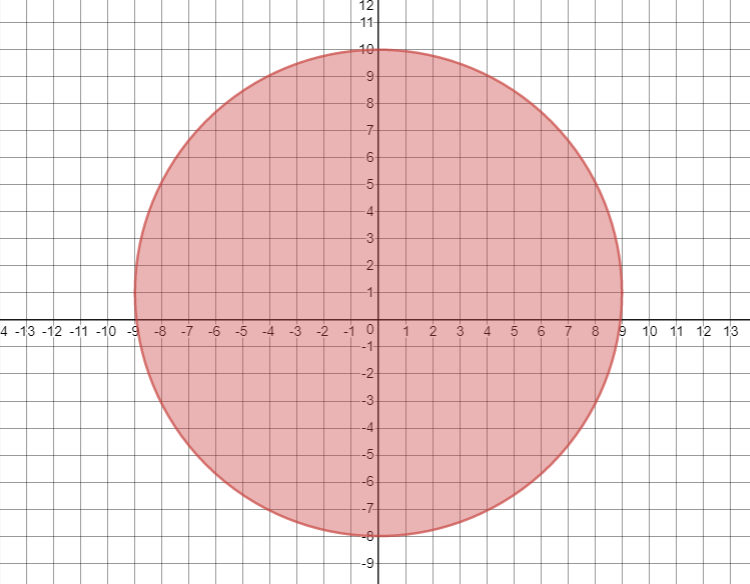
\includegraphics[scale=0.65]{01-NumerosComplejos/complejos7d.png}
	\end{center}
	\pagebreak
	\subsubsection{7h}
	$\mathrm{h)}\; \displaystyle{\left\vert \frac{z-5}{4+\imj} \right\vert < 1}$
	
	Empezamos diviendo el módulo, aplicando propiedades:
	$$\displaystyle{\frac{\left\vert z-5 \right\vert}{\left\vert 4+\imj \right\vert} < 1}$$
	\begin{center}
		Calculamos el módulo en el denominador y además reemplacemos la $z$ del numerador y agrupemos:
	\end{center}
	$$\displaystyle{\frac{\left\vert (x-5)+y\imj \right\vert}{{\sqrt{4^2+1^2}}}<1}$$
	$$\displaystyle{\frac{\left\vert (x-5)+y\imj \right\vert}{{\sqrt{17}}}<1}$$
	\begin{center}
		Aplicamos módulo al numerador y pasamos multiplicando el denominador:
	\end{center}
	$$\displaystyle{\sqrt{ (x-5)^{2}+y^{2} } < \sqrt{17}}$$
	\begin{center}
		\fcolorbox{black}{yellow}{$\displaystyle{(x-5)^2 + y^2 < 17}$}
	\end{center}
	\vspace*{0.5cm}
	Esto es el interior de una circunferencia de radio $\sqrt{17}$ con centro en (5;0), sin incluir el borde.
	La gráfica de esta circunferencia sería:
	\begin{center}
		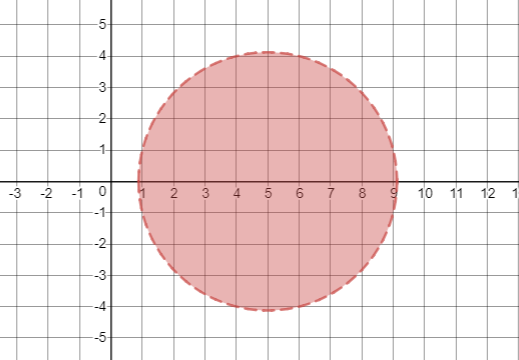
\includegraphics[scale=0.75]{01-NumerosComplejos/complejos7h.png}
	\end{center}
	
	\subsection{Ejercicios 8fgi}
	
	Resuelva las siguientes ecuaciones en $\mathbb{C}$ en forma binómica:
	
	\subsubsection{8f}
	$\mathrm{f)} \; z^2-(2+\imj)z+(-1+7\imj)=0$
	
	Para resolver este tipo de ejercicios vale aplicar la fórmula resolvente de las ecuaciones cuadráticas, hacemos de cuenta que $z$ es la $x$ que usamos siempre.\\
	En estos casos, aplicamos lo mismo de siempre:
	$$a=1 \; \; \; \; b=-(2+\imj) \; \; \; \; c=-1+7\imj$$
	$$\displaystyle{z_{1,2}=\frac{2+\imj \pm \sqrt{\left( -(2+\imj) \right)^2 - 4 \cdot 1 \cdot (-1+7\imj)}}{2\cdot 1}}$$
	$$\displaystyle{z_{1,2}=\frac{2+\imj \pm \sqrt{4 + 4\imj - 1 + 4 - 28\imj}}{2}}$$
	$$\displaystyle{z_{1,2}=\frac{2+\imj \pm \sqrt{7 - 24\imj}}{2}}$$
	Ahora, concentremonos únicamente en la raíz que está en el numerador y recordemos las definiciones necesarias para resolver una raíz de un número complejo en forma binómica.
	
	\begin{center}
		Sea $z=a+b\imj$ un número complejo, queremos calcular $\sqrt{z}$, así que llamemos $\sqrt{z}=w$, donde $w$ es otro número complejo, de la forma $w=x+y\imj$. Para calcular $x$ e $y$, tenemos las formulas:
	\end{center}
	$$x=\pm\sqrt{\frac{|z|+a}{2}}$$
	$$y=\pm\sqrt{\frac{|z|-a}{2}}$$
	
	\begin{center}
		Hacemos el cálculo del módulo: $|z|=\sqrt{7^2+24^2}=25$
		
		Reemplazamos en las fórmulas:
	\end{center}
	$$x=\pm\sqrt{\frac{25+7}{2}}=\pm\sqrt{16}=4$$
	$$y=\pm\sqrt{\frac{25-7}{2}}=\pm\sqrt{9}=3$$
	Ahora tenemos que tener en cuenta que, para elegir los signos de $x$ e $y$ (por los $\pm$), hay que fijarse el signo de la parte imaginaria de $z$. Si $b<0$ tomamos signos alternados. En cambio, si $b>0$, tomamos signos iguales.
	
	En este caso vamos a tomar signos alternados por que $b<0$
	
	Entonces tendremos: $w_{1}=4-3\imj\;\wedge\;w_{2}=-4+3\imj$
	
	Ahora, para seguir con el ejercicio vale la pena aclarar algo con los valores obtenidos y el $\pm$ que es propio de la fórmula de la resolvente. 
	
	Es una redundancia hacer las cuentas dos veces (una para el más, y otra para el menos) para los DOS valores de $w$ hallados. Ya que con el $\pm$ estaremos cambiando los signos de una solución para que nos termine dando la otra, esto es lo siguiente:
	
	\begin{center}
		Si primero usamos $w_{1}$ vamos a ver que tenemos $\displaystyle{\frac{(2+\imj)+(4-3\imj)}{2}}$ si entramos por el $+$.
		
		Y si entramos por el $-$ vamos a tener $\displaystyle{\frac{(2+\imj)-(4-3\imj)}{2}}$
		
		Distribuyendo el $-$ nos queda $\displaystyle{\frac{(2+\imj)+(-4+3\imj)}{2}}$ . Y si nos damos cuenta, ¡el valor que nos quedó en el segundo paréntesis es $w_{2}$! Si realizaramos el mismo procedimiento con $w_{2}$ , al entrar por el $-$ nos quedaría $w_{1}$.
	\end{center}
	En conclusión nos conviene tomar dos caminos:
	\begin{itemize}
		\item Tomamos ambos valores $w_{1}$ y $w_{2}$ y los pasamos únicamente por el $+$ del $\pm$ de la resolvente.
		\item Tomamos uno de los dos valores $w_{1}$ ó (excluyente) $w_{2}$ y lo pasamos por ambas operaciones ($+$ y $-$) del $\pm$ de la fórmula resolvente.
	\end{itemize}
	
	Dicho todo esto, yo voy a aplicar la primera regla para terminar los cálculos:
	
	$$z_{1}=\frac{(2+\imj)+(4-3\imj)}{2}=\frac{6-2\imj}{2}=3-\imj$$
	$$z_{2}=\frac{(2+\imj)+(-4+3\imj)}{2}=\frac{-2+4\imj}{2}=-1+2\imj$$
	
	Por lo tanto nuestras soluciones son finalmente:
	\fcolorbox{black}{yellow}{$z_{1}=3-\imj\;\;\;\;z_{2}=-1+2\imj$}
	
	\subsubsection{8g}
	$\mathrm{g)} \; z^{2}-(5+3\imj)z+(4+20\imj)=0$
	
	Procedemos de la misma manera que el ejercicio anterior:
	$$\displaystyle{z_{1,2}=\frac{5+3\imj \pm \sqrt{(5+3\imj)^2-4\cdot 1 \cdot (4+20\imj)}}{2\cdot 1}}$$
	$$\displaystyle{z_{1,2}=\frac{5+3\imj \pm \sqrt{25+30\imj-9 -16-80\imj}}{2}}$$
	$$\displaystyle{z_{1,2}=\frac{5+3\imj \pm \sqrt{-50\imj}}{2}}$$
	\begin{center}
		Resolvemos la raíz:
	\end{center}
	$$x=\pm \sqrt{\frac{50+0}{2}}=\pm5$$
	$$y=\pm \sqrt{\frac{50-0}{2}}=\pm5$$
	\begin{center}
		Como $b<0$ tomamos signos alternados:
	\end{center}
	$$w_{1}=5-5\imj\;\;\;\;w_{2}=-5+5\imj$$
	\begin{center}
		Los usamos en la resolvente:
	\end{center}
	$$z_{1}=\frac{5+3\imj+5-5\imj}{2}=5-\imj$$
	$$z_{2}=\frac{5+3\imj-5+5\imj}{2}=4\imj$$
	
	Finalmente las soluciones son: \fcolorbox{black}{yellow}{$z_{1}=5-\imj\;\;\;\;z_{2}=4\imj$}
	
	\subsubsection{8i}
	$\mathrm{f)}\; z^4+16=0$
	
	Primero, hacemos un pequeño pasaje de términos y sacamos la raíz cuarta:
	$$\displaystyle{z=\pm\sqrt[4]{-16}}$$
	Para ayudarnos a resolver con herramientas que conozcamos (no podemos sacar una raíz cuarta, al menos no con métodos convencionales) vamos a reescribir la raíz cuarta como la raíz de la raíz cuadrada:
	$$z=\pm\sqrt{\pm\sqrt{-16}}$$
	
	\begin{center}
		Si nos concentramos en la raíz más interior, podemos también reescribirla como:
	\end{center}
	$$\sqrt{-16}=\sqrt{16}\sqrt{-1}$$
	\begin{center}
		Pero sabemos que $\sqrt{-1}=\imj$, entonces tenemos:
	\end{center}
	$$z=\sqrt{4\imj}$$
	$$z=\pm\sqrt{\pm4\imj}$$
	\begin{center}
		Partimos el problema en dos:
	\end{center}
	\begin{center}
		\begin{tabular}{c  |  c}
			$z=\pm \sqrt{4\imj}$ & $z=\pm\sqrt{-4\imj}$ \\[0.5cm] \hline
			$\displaystyle{x=\pm \sqrt{\frac{4}{2}}=\pm\sqrt{2}}$ & $\displaystyle{x=\pm \sqrt{\frac{4}{2}}=\pm \sqrt{2}}$ \\[0.5cm]
			$\displaystyle{y=\pm \sqrt{\frac{4}{2}}=\pm \sqrt{2}}$ & $\displaystyle{y=\pm \sqrt{\frac{4}{2}}=\pm \sqrt{2}}$ \\ \hline
			Tomo signos iguales ($b>0$) & Tomo signos alternados ($b<0$) \\[0.25cm]
			\fcolorbox{black}{yellow}{$z_{1}=\sqrt{2}+\sqrt{2}\imj$} & \fcolorbox{black}{yellow}{$z_{3}=\sqrt{2}-\sqrt{2}\imj$} \\[0.25cm]
			\fcolorbox{black}{yellow}{$z_{2}=-\sqrt{2}-\sqrt{2}\imj$} & \fcolorbox{black}{yellow}{$z_{4}=-\sqrt{2}+\sqrt{2}\imj$}
		\end{tabular}
	\end{center}
	\subsection{Ejercicio 9}
	\subsubsection{9a}
	a) Escriba una ecuación polinómica de grado 2 con coeficientes complejos tal que una raíz sea real y la otra compleja no real.
	
	Para resolver este ejercicio recordemos la ecuación de un polinomio de segundo grado:
	$$mz^{2}+nz+o=0$$
	
	Este polinomio tendrá dos raíces $z_{1}$ y $z_{2}$.\\
	Recordemos también las relaciones entre las raíces:
	$$z_{1}+z_{2}=-\frac{n}{m} \;\;\;\;\;\; z_{1} \cdot z_{2} = \frac{o}{m} $$
	
	Por lo tanto, trabajemos con la ecuación original. Vamos a elegir una ecuación reducida o mónica y dividamos a nuestra expresión por $m$.
	
	$$\frac{m}{m}z^2+\frac{n}{m}z+\frac{o}{m}=0$$
	$$z^2+\frac{n}{m}+\frac{o}{m}=0$$
	\begin{center}
		Tengamos en cuenta que $m\neq0$.
	\end{center}
	Entonces, según el enunciado vamos a proponer las dos soluciones genéricas:
	$$z_{1}=a\;\;\;\;\;\;z_{2}=b+c\imj$$
	Teniendo en cuenta las relaciones entre raíces mencionadas arriba, podemos dar la solución genérica, ya que tenemos igualdades que podemos utilizar.
	\begin{center}
		\fcolorbox{black}{yellow}{$z^{2}+(a+b+c\imj)z+a(b+c\imj)=0$}
	\end{center}
	
	
	\subsubsection{9b}
	b) ¿Sería posible lo mismo si los coeficientes fueran todos reales? ¿Por qué? \\
	No, no sería posible. Esto es debido a que siempre que los coeficientes sean \textbf{TODOS} reales, en caso de que una raíz sea compleja no real, entonces su conjugada también es raíz, es decir, las complejas vienen de a pares.
	\section{Forma polar}
	\subsection{Ejercicio 11b}
	Calcule el resultado de las siguientes operaciones en forma polar:
	
	b) Dados: $\;\;$\resizebox{2.25cm}{!}{$z_{1}=16e^{\frac{5\pi}{6}\imj}$} $\;\;$ y $\;\;$ \resizebox{2.25cm}{!}{$z_{2}=2e^{\frac{\pi}{4}\imj}$} $\;\;$ Halle: \resizebox{2.25cm}{!}{$z=\frac{z_{1}}{{z_{2}}^{3}}$}
	
	Bien, tenemos los números $z_{1}=\left[ 16;\frac{5\pi}{6} \right]$ y $z_{2}=\left[ 2; \frac{\pi}{4} \right] $
	
	Empecemos haciendo la potenciación del número $z_{2}$.
	
	Para ello, recordemos que la potenciación de un número complejo en forma polar es:\\
	Dado un número $z=\left[ \rho;\phi \right] $ entonces $z^{n}=\left[\rho^{n};\, n\phi \right]$
	
	Por lo tanto ${z_{2}}^3= \left[2^{3}; 3\cdot \frac{\pi}{4}\right]=\left[8; \frac{3\pi}{4}\right]$
	
	Entonces: $z=\frac{\left[16; \frac{5\pi}{6}\right]}{\left[8; \frac{3\pi}{4}\right]}$
	
	Por último, faltaría hacer el cociente. Recordemos como se hace.
	Dados $z_{1}=\left[\rho_{1};\phi_{1}\right]$ y $z_{2}=\left[\rho_{2}; \phi_{2}\right]$.\\
	Entonces z=$\frac{z_{1}}{z_{2}}=\left[\frac{\rho_{1}}{\rho_{2}}; \phi_{1}-\phi_{2}\right]$
	
	Procedemos entonces para nuestro caso:
	
	$z=\frac{\left[16;\frac{5\pi}{6}\right]}{\left[8;\frac{3\pi}{4}\right]}=\left[\frac{16}{8}; \frac{5\pi}{6}-\frac{3\pi}{4}\right] =$ \fcolorbox{black}{yellow}{$\left[2;\frac{\pi}{12}\right]$}
	\section{Raíces n-ésimas}
	\subsection{Ejercicio 13b}
	Resuelva las siguientes ecuaciones en $\mathbb{C}$ en forma polar:
	
	b) $z^4=1+\imj$
	
	Para resolver este ejercicio, tengamos en cuenta que la radicación de un número complejo en forma polar se realiza:
	
	Dado un número complejo en forma polar $z=\left[\rho;\phi\right] entonces \sqrt[n]{z}=w$ , donde $w$ es otro número complejo, en forma polar, de la forma $w=\left[r;\theta\right]$.
	
	Para $w$, sus componentes se calculan:\\
	$r=\sqrt[n]{\rho} \: \wedge \: \theta=\frac{\phi +2k\pi}{n}$ donde $k=0,1,2,\cdots,n-1$
	
	Teniendo en cuenta todo esto, procedamos a calcular las raíces de la ecuación.
	
	$z=\sqrt[4]{1+\imj} \;\;\;$ Esta operación nos va a producir las $w_{k}$ soluciones, donde $k\in{0,1,2,3}$
	
	Para poder realizar esto, necesitamos pasar el número a forma polar:
	
	$\left(1,1\right)\;$\textrightarrow$\;\left[\sqrt{2};\frac{\pi}{4}\right]$
	
	Ya que tenemos nuestro número en forma polar, es momento de calcular las $w_{k}$.\\
	$w_{0}=\left[\sqrt[4]{\sqrt{2}};\frac{\frac{\pi}{4}+2\cdot0\pi}{4}\right]=$\fcolorbox{black}{yellow}{$\left[\sqrt[8]{2};\frac{\pi}{16}\right]$}\\
	\fcolorbox{black}{yellow}{$w_{1}=\left[\sqrt[8]{2};\frac{9\pi}{16}\right]$}\\
	\fcolorbox{black}{yellow}{$w_{2}=\left[\sqrt[8]{2};\frac{17\pi}{16}\right]$}\\
	\fcolorbox{black}{yellow}{$w_{3}=\left[\sqrt[8]{2};\frac{25\pi}{16}\right]$}
	\section{Logaritmo natural y exponenciales complejas}
	\subsection{Ejercicios 17bc}
	Halle $\ln z$ para:
	\subsubsection{17b}
	b) $z=-4$
	
	Para empezar a resolver este ejercicio vale aclarar que los logaritmos de números negativos no tienen solución en los reales, sin embargo si la tienen en el campo de los números complejos.
	
	Así que recordemos como se calculan:
	
	Dado un número complejo en forma polar $z=\left[\rho;\phi\right]$. \\
	Entonces $\ln z = \ln(\rho) + \imj\left(\phi + 2k\pi\right)$. Donde para $k=0$ se define al resultado como el valor principal de $\ln z$. También, ¡notemos que el resultado es un número complejo en forma binómica!
	
	Entonces, para este ejercicio en particular, empecemos pasando nuestro número a forma polar:\\
	$\left(-4, 0\right)\;$ \textrightarrow $\;\left[4;\pi\right]$
	
	Ahora saquemos el logaritmo natural para concluir el ejercicio: \\
	\fcolorbox{black}{yellow}{$\ln z = \ln(4) + \imj\left(\pi + 2k\pi\right)$}
	
	\subsubsection{17c}
	c) $z=-e^{\imj \pi}$
	
	En este ejercicio hay que tener cuidado de NO considerar el $-1$ como el módulo del número complejo. Tener presente que el módulo siempre es un número positivo, a lo sumo $0$.\\
	En este caso, tenemos que considerar una multiplicación de números complejos. El número complejo $-1$ y el número complejo $e^{\imj\pi}$.\\
	Entonces $z=\left[1;\pi\right]\cdot\left[1;\pi\right]=\left[1;2\pi\right]\equiv\left[1;0\right]$
	
	Por último, \fcolorbox{black}{yellow}{$\ln z = \ln(1) + \imj(0+2k\pi)=2k\pi\imj$}
	
	\textbf{Manera alternativa de llegar al resultado} (usando la identidad de Euler)
	
	Partiendo de la fórmula de Euler: $e^{\imj x}=\cos x + \imj \sen x$\\
	En particular si hacemos $x=\pi$: $\;\;e^{\imj \pi} = \cos \pi + \imj \sen \pi \implies e^{\imj \pi}=-1 \implies \cdots$ \\ $$\boxed{e^{\imj \pi} + 1 = 0}$$
	
	Obtuvimos la Identidad de Euler (la cual es famosísima por su belleza y los números que relaciona). Luego, si la acomodamos convenientemente: $-e^{\imj\pi}=1$
	
	Tenemos el mismo número del enunciado, por lo que reemplazamos: $z=1=\left[1;0\right]$ (en forma polar).
	
	Por último, se procede igual que como hicimos antes, llegando al mismo resultado.
	\subsection{Ejercicios 19ce}
	Halle el valor principal de $z$ que verifique las siguientes igualdades
	\subsubsection{19c}
	c) $z=\sqrt[1+\imj]{\imj}$
	
	Empecemos expresando la igualdad de forma conveniente:\\
	$z=\imj^{\frac{1}{1+\imj}}$
	
	Ahora sigamos operando:\\
	$\ln z = \frac{1}{1+\imj} \ln(j)$
	
	$\ln z = \frac{1}{1+\imj} \ln\left(\left[1; \frac{\pi}{2}\right]\right)=\frac{1}{1+\imj}\left(\ln(1)+\imj\left(\frac{\pi}{2}+2k\pi\right)\right) \;\;\;$ Como nos están pidiendo el VP, hacemos $k=0$
	
	$\ln z = \frac{1}{1+\imj}\cdot \frac{\pi}{2}\imj= \frac{\frac{\pi}{2}\imj}{1+\imj}=\frac{\frac{\pi}{2}\imj}{1+\imj}\cdot\frac{1-\imj}{1-\imj}=\frac{\frac{\pi}{2}+\frac{\pi}{2}\imj}{2}=\boxed{\frac{\pi}{4}+\frac{\pi}{4}\imj}$
	
	¡Pero cuidado! Nos están pidiendo el VP de $z$, y nosotros arriba obtuvimos el VP del $\ln z$. Por lo tanto, hay que seguir operando:
	
	$e^{\ln z} = e^{\frac{\pi}{4}+\frac{\pi}{4}\imj}\implies z=e^{\frac{\pi}{4}}e^{\frac{\pi}{4}\imj} \;\;\;$ De esta manera, el número es $z=\left[e^{\frac{\pi}{4}};\frac{\pi}{4}\right]$.
	
	Para llegar al resultado de la guía, hay que seguir operando y usar la fórmula de Euler.
	
	$z=e^{\frac{\pi}{4}}\cdot\left(\cos\left(\frac{\pi}{4}\right)+\imj \sen\left(\frac{\pi}{4}\right)\right)=e^{\frac{\pi}{4}}\cdot\left(\frac{\sqrt{2}}{2}+\frac{\sqrt{2}}{2}\imj\right) \implies$ \fcolorbox{black}{yellow}{$z=e^{\frac{\pi}{4}}\frac{\sqrt{2}}{2}(1+\imj)$}
	
	\subsubsection{19e}
	e) $\sqrt[z]{\frac{1-\sqrt{3}\imj}{2}}=\frac{1+\sqrt{3}\imj}{2\imj}$
	
	Operemos:\\
	$\left(\frac{1-\sqrt{3}\imj}{2}\right)^{\frac{1}{z}}=\frac{1+\sqrt{3}\imj}{2\imj}\cdot\frac{\imj}{\imj} \implies \left(\frac{1-\sqrt{3}\imj}{2}\right)^{\frac{1}{z}}=\frac{\sqrt{3}-\imj}{2}$
	
	Aplicamos logaritmo a ambos lados:
	
	$\frac{1}{z}\ln\left(\frac{1}{2}-\frac{\sqrt{3}}{2}\imj\right)=\ln\left(\frac{\sqrt{3}}{2}-\frac{1}{2}\imj\right) \;\;\;$ Pasamos a polar: $\left(\frac{1}{2},- \frac{\sqrt{3}}{2}\right)$\textrightarrow$\left[1;\frac{5\pi}{3}\right]\;\;\;\left(\frac{\sqrt{3}}{2},-\frac{1}{2}\right)$\textrightarrow$\left[1;\frac{11\pi}{6}\right]$
	
	$\frac{1}{z}\ln\left(\left[1;\frac{5\pi}{3}\right]\right)=\ln\left(\left[1;\frac{11\pi}{6}\right]\right)\implies\frac{1}{z}\cdot\frac{5\cancel{\pi}}{3}\cancel{\imj}=\frac{11\cancel{\pi}}{6}\cancel{\imj}\implies\frac{1}{z}=\frac{3\cdot11}{6\cdot5}\implies\cdots$
	
	\fcolorbox{black}{yellow}{$z=\frac{10}{11}$}
	\section{Ejercicios combinados}
	\subsection{Ejercicio 20B}
	Halle analíticamente y grafique los conjuntos (Considere: $z=x+\imj y$)
	
	$\mathrm{B}=\left\lbrace z\in\mathbb{C} / z^{5}+4-4\imj=0 \, \wedge \, 5\left|z\right|^{2}+3\mathrm{Re}\left(z^{2}\right) \leq 8 \right\rbrace$
	
	Resolvamos de a partes las soluciones
	
	Empecemos con $z^{5}+4-4\imj=0$ \textrightarrow $z=\sqrt[5]{-4+4\imj}$
	
	Hacemos pasaje a polar: $\left(-4, 4\right)$ \textrightarrow $\left[4\sqrt{2};\frac{3\pi}{4}\right]$
	
	Entonces las $w_{k}$ serán:
	
	$\boxed{\;\; w_{0}=\left[\sqrt{2}; \frac{3\pi}{20}\right] \;\; w_{1}=\left[\sqrt{2}; \frac{11\pi}{20}\right] \;\; w_{2}=\left[\sqrt{2}; \frac{19\pi}{20}\right] \;\; w_{3}=\left[\sqrt{2}; \frac{27\pi}{20}\right] \;\; w_{4}=\left[\sqrt{2}; \frac{7\pi}{4}\right] \;\;}$\vspace{0.5cm}\\
	
	Para la segunda parte: $5\left|z\right|^{2}+3\mathrm{Re}\left(z^{2}\right) \leq 8$
	
	$5\left(x^2+y^2\right)+3\mathrm{Re}\left(x^2+2xy\imj-y^2\right)\leq8\implies8x^2+2y^2\leq8\;\;$ Es una elipse de eje $y$ con centro en $\left(0,0\right)$ y su interior.
	
	A continuación, podemos realizar la gráfica de los puntos y de la elipse:

	\begin{center}
		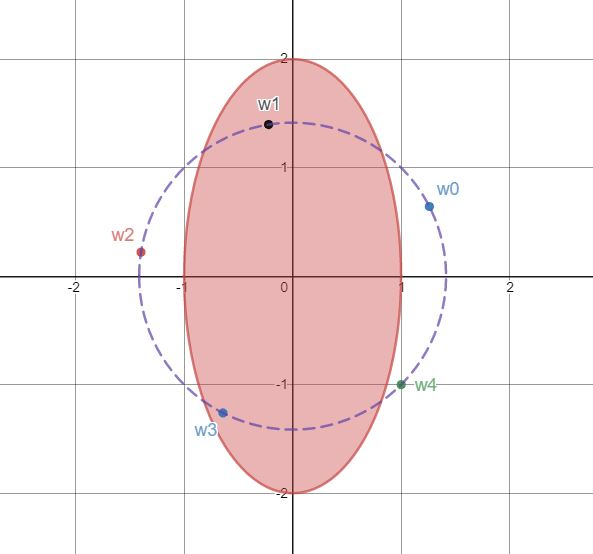
\includegraphics[scale=0.8]{01-NumerosComplejos/20b.JPG}
	\end{center}

	De esta manera podemos visualizar rápidamente cuál es la intersección de la solución de los dos conjuntos. Hay algunos números para los cuales no tendremos dudas que son o no son parte de la intersección (considerando que lo hacemos en una hoja, y no con un graficador, como yo), y en cambio, si queremos asegurarnos de otros números como el $w_{3}$ o el $w_{4}$, donde quizás en un gráfico hecho a mano no es muy clara la intersección, siempre podemos pasar los números del primer conjunto a binómica y luego verificar si cumplen la desigualdad del segundo.
	
	Por último, el conjunto solución es \fcolorbox{black}{yellow}{$\mathrm{B}=\left\lbrace \left[\sqrt{2};\frac{11\pi}{20}\right], \left[\sqrt{2};\frac{27\pi}{20}\right] \right\rbrace$}
	\pagebreak
	\section{Superposición de señales senoidales de igual frecuencia}
	\subsection{Ejercicio 22d}
	Dadas las funciones $f$ y $g$ obtenga la función $f+g$ utilizando fasores:
	
	d) $f(t)=4\cos(3t) \;\;\;$ y $\;\;\;g(t)=6\sen(3t)$
	
	Primero hay que considerar que ambas funciones deben ser del mismo tipo. Es decir, no podemos sumar senos y cosenos. Sino, que ambas deben ser senos o bien ambas cosenos.
	
	Transformemos la función $g$.
	
	La desfasamos, teniendo en cuenta que $\sen(\theta)=\cos\left(\theta-\frac{\pi}{2}\right)$
	
	Por ende, en nuestro caso quedaría: $g(t)=6\cos\left(3t-\frac{\pi}{2}\right)$
	
	$F_{f}=4e^{0j}=4 \;\;\; F_{g}=6e^{-\frac{\pi}{2}\imj}$
	
	Pasamos los fasores a forma binómica:
	$F_{f}=4 \;\;\; F_{g}=-6\imj$
	
	Los sumamos:
	$F_{f}+F_{g}=4-6\imj$
	
	Sacamos módulo y argumento de la suma de los fasores:\\
	$\boxed{A=\sqrt{4^{2}+6^{2}}=2\sqrt{13}\approx7.21} \;\;\;\;\;\;\;\; \boxed{\phi=\arctan\left(\frac{-6}{4}\right)=-0.98}$
	
	Para terminar, vamos a escribir nuestra señal resultante. Tener en cuenta que la frecuencia es la misma y la función también (es decir, en este caso sería un coseno y la frecuencia es 3). En caso de que la frecuencia no coincida, NO se puede resolver el ejercicio por fasores. Se debería usar otro método, como por ejemplo la Serie de Fourier.
	
	\fcolorbox{black}{yellow}{$(f+g)(t)=7.21\cos\left(3t-0.98\right)$}
	
\end{document}
